\chapter{TỔNG QUAN}
\section{Các nghiên cứu có liên quan ngoài nước}
Hiện nay tại các nước phát triển thì chiếu sáng nhân tạo là một vấn đề được rất nhiều công ty, tổ chức quan tâm và nghiên cứu. Chiếu sáng nhân tạo phục vụ các nhu cầu khác nhau: như trồng cây trong nhà kính, chiếu sáng các văn phòng, các phòng học… Tuy phục vụ các nhu cầu khác nhau nhưng điểm chung giữa các nghiên cứu ấy đều tập trung điều chỉnh cường độ ánh sáng và độ rọi lên bề mặt cần chiếu sáng.

Tại Farmertyler, một công ty tư vấn nông nghiệp chuyên về nông nghiệp đô thị, thủy canh, canh tác thẳng đứng và sản xuất nhà kính, ánh sáng được điều chỉnh và lựa chọn màu sắc phù hợp để kích thích và làm cho cây trồng phát triển và sinh trưởng nhanh. (Hình~\ref{fig:nhakinhtrongrau})
\begin{center}
    \begin{figure}[!htp]
    \begin{center}
     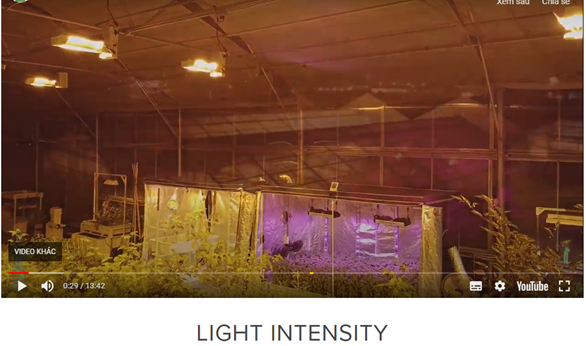
\includegraphics[scale=0.9]{Chapters/Chapter2/ImagesChapter2/Nhakinhtrongrau}
    \end{center}
    \caption{Cân bằng ánh sáng trong nhà kính trồng rau}
    \label{fig:nhakinhtrongrau}
    \end{figure}
\end{center}

Theo như bài nghiên cứu của tác giả: Sanaz Sanami thuộc Payame Noor University với bài nghiên cứu: “The Impact of Indoor Lighting on Students’ Learning Performance in Learning”. Bài nghiên cứu chỉ ra cho chúng ta thấy tác động của chiếu sáng trong phòng ảnh hưởng đến hiệu quả học tập của học sinh.

Hay như một bài nghiên cứu của Đại học Monash về ánh sáng nhân tạo tới nhịp sinh học thì PGS Cain cho biết: “Sự cân bằng âm và dương cũng là sự cân bằng giữa ánh sáng và bóng tối. Và sự cân bằng này rất quan trọng đối với việc điều tiết hệ thống sinh lý học của chúng ta. Ánh sáng nhân tạo phá vỡ nhịp hoạt động này, làm rối loạn giấc ngủ, ảnh hưởng đến sức khỏe và là nguyên nhân dẫn đến nhiều bệnh mãn tính hơn”.

\section{Các nghiên cứu có liên quan trong nước}
Hiện nay trong nước thì vấn đề về chiếu sáng trong phòng cũng chưa được quan tâm nhiều. Ở các phòng học và các công xưởng thì vấn đề chiếu sáng chỉ dừng ở mức độ chiếu đủ độ sáng. (Hình~\ref{fig:nhakho})
\begin{center}
    \begin{figure}[!htp]
    \begin{center}
     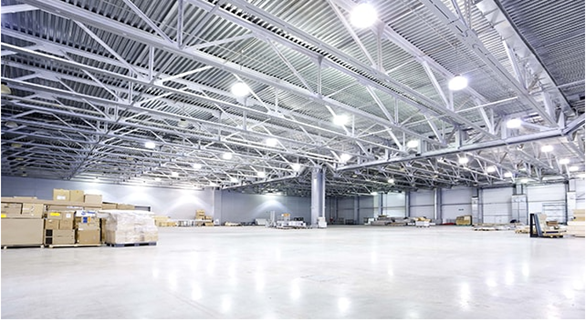
\includegraphics[scale=0.9]{Chapters/Chapter2/ImagesChapter2/Nhakho}
    \end{center}
    \caption{Chiếu sáng trong nhà kho}
    \label{fig:nhakho}
    \end{figure}
\end{center}

Ở các phòng công nghiệp thì ánh sáng được lắp và phân bố đều nhưng chỉ đảm bảo độ sáng chứ chưa có chuyên sâu về mức độ đảm bảo sức khỏe.

Công ty FSIVN, chuyên cung cấp các giải pháp thiết kế chiếu sáng trường học. Hình dưới là giải pháp của công ty cho một phòng học với ánh sáng trải đều, đèn điện có máng che đèn điện lắp so le và không có loáng của quạt. (Hình~\ref{fig:lophoc})

Từ hình ảnh trên chúng ta cũng thấy được ưu điểm của phương pháp này là ánh sáng của căn phòng luôn đạt được độ sáng chênh lệch và dao động từ 300-500 lux. Nhưng nhược điểm của nó là có thể thấy vào những ngày thời tiết khác nhau cường độ ánh sáng bên ngoài tác động vào thì ánh sáng trong phòng sẽ khác, có nơi cường độ ánh sáng cao hơn mức cho phép và cũng có những nơi không đạt được độ sáng cần thiết.
\begin{center}
    \begin{figure}[!htp]
    \begin{center}
     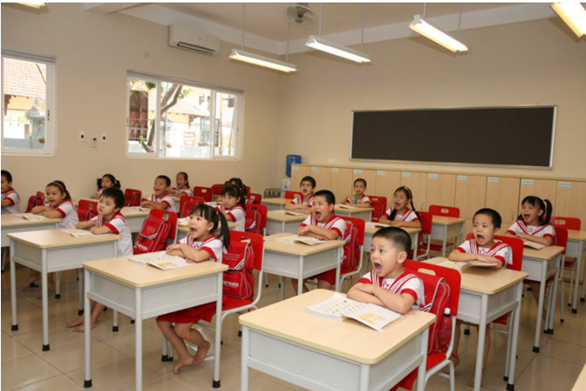
\includegraphics[scale=0.9]{Chapters/Chapter2/ImagesChapter2/Lophoc}
    \end{center}
    \caption{Chiếu sáng trong lớp học}
    \label{fig:lophoc}
    \end{figure}
\end{center}

\section{Hướng nghiên cứu và phát triển}
Từ các bài nghiên cứu ở ngoài nước và trong nước thì chúng ta có thể thấy tầm quan trọng của ánh sáng nhân tạo hiện nay rất quan trọng. Tác động tích cực và tiêu cực của nó đối với con người và sinh vật rất lớn.

Nhận thấy tính quan trọng và cấp thiết của vấn đề. Nhóm chúng em lựa chọn nghiên cứu “Hệ thống cân bằng ánh sáng trong phòng kín” với mục đích là đề ra là tạo ra hệ thống cung cấp đủ ánh sáng trong phòng, cung cấp ánh sáng với độ rọi phù hợp. Hệ thống được xây dựng với định hướng nghiên cứu:
\begin{itemize}
\item Cung cấp ánh sáng trải đều trên diện tích chiếu sáng.
\item Hệ thống tự điều chỉnh được bố cục đèn.
\item Hệ thống tự đo và điều chỉnh cường độ ánh sáng khi có tác động ánh sáng khác từ bên ngoài.
\item Báo cáo liên tục cho người dùng độ sáng của đèn.
\item Đưa ra khuyến nghị khi ánh sáng trong phòng thay đổi. 
\end{itemize}

